%%%%%%%%%%%%%%%%%%%%%%%%%%%%%%%%%%%%%%%%%%%%%%%%%%%%%%%%%%%%%%%%%%%%%%%%%%%%%%%%%%%%%%%%%%%%%%%%%
%
% Document:      DM  operations product tree
%
%%%%%%%%%%%%%%%%%%%%%%%%%%%%%%%%%%%%%%%%%%%%%%%%%%%%%%%%%%%%%%%%%%%%%%%%%%%%%%
\documentclass{article}
\usepackage{times,layouts}
\usepackage{tikz,hyperref,amsmath}
\usetikzlibrary{positioning,arrows,shapes,decorations.shapes,shapes.arrows}
\usetikzlibrary{backgrounds,calc}
\usepackage[paperwidth=185.4cm,paperheight=15.3cm,
left=-2mm,top=3mm,bottom=0mm,right=0mm,
noheadfoot,marginparwidth=0pt,includemp=false,
textwidth=30cm,textheight=50mm]{geometry}
\newcommand\showpage{%
\setlayoutscale{0.5}\setlabelfont{\tiny}\printheadingsfalse\printparametersfalse
\currentpage\pagedesign}
\hypersetup{pdftitle={DM products }, pdfsubject={Diagram illustrating the
products in LSST DM }, pdfauthor={ William O'Mullane}}
\tikzstyle{tbox}=[rectangle,text centered, text width=30mm]
\tikzstyle{wbbox}=[rectangle, rounded corners=3pt, draw=black, top color=blue!50!white, bottom color=white, very thick, minimum height=12mm, inner sep=2pt, text centered, text width=30mm]
\tikzstyle{pbox}=[rectangle, rounded corners=3pt, draw=black, top color=yellow!50!white, bottom color=white, very thick, minimum height=35pt, inner sep=2pt, text centered, text width=35mm]
\tikzstyle{abox}=[rectangle, rounded corners=3pt, draw=black, top color=green!50!white, bottom color=white, very thick, minimum height=35pt, inner sep=2pt, text centered, text width=35mm]
\tikzstyle{tbox}=[rectangle, rounded corners=3pt, draw=black, top color=blue!50!white, bottom color=white, very thick, minimum height=35pt, inner sep=2pt, text centered, text width=35mm]
\tikzstyle{gbox}=[rectangle, rounded corners=3pt, draw=black, top color=cyan!50!white, bottom color=white, very thick, minimum height=35pt, inner sep=2pt, text centered, text width=35mm]
\tikzstyle{pline}=[-, thick]
\begin{document}
\begin{tikzpicture}[node distance=0mm]
\node (3-felis) [pbox,] {\textbf{Felis} };
\node [below right] at (3-felis.north west) {\small \color{blue}Product} ;
\node (3-meta) [pbox,right=1mm of 3-felis] {\textbf{Metadata} };
\node [below right] at (3-meta.north west) {\small \color{blue}Activity} ;
\node (3-bps) [pbox,right=15mm of 3-meta] {\textbf{BPS} };
\node [below right] at (3-bps.north west) {\small \color{blue}Product} ;
\node (3-butler) [pbox,right=1mm of 3-bps] {\textbf{Butler} };
\node [below right] at (3-butler.north west) {\small \color{blue}Product} ;
\node (3-ctrl) [pbox,right=1mm of 3-butler] {\textbf{Control Interface} };
\node [below right] at (3-ctrl.north west) {\small \color{blue}Product} ;
\node (3-spinter) [pbox,right=46mm of 3-ctrl] {\textbf{Pipeline interfaces} };
\node [below right] at (3-spinter.north west) {\small \color{blue}Product} ;
\node (3-ocps) [pbox,right=31mm of 3-spinter] {\textbf{OCPS} };
\node [below right] at (3-ocps.north west) {\small \color{blue}Product} ;
\node (3-prompt) [pbox,right=1mm of 3-ocps] {\textbf{Prompt f/ w} };
\node [below right] at (3-prompt.north west) {\small \color{blue}Product} ;
\node (3-Backbone) [pbox,right=15mm of 3-prompt] {\textbf{Data Backbone} };
\node [below right] at (3-Backbone.north west) {\small \color{blue}Activity} ;
\node (3-Backups) [pbox,right=1mm of 3-Backbone] {\textbf{Backups} };
\node [below right] at (3-Backups.north west) {\small \color{blue}Activity} ;
\node (3-Bulk) [pbox,right=1mm of 3-Backups] {\textbf{Bulk Download} };
\node [below right] at (3-Bulk.north west) {\small \color{blue}Activity} ;
\node (3-Consol) [pbox,right=1mm of 3-Bulk] {\textbf{Consolidated DB} };
\node [below right] at (3-Consol.north west) {\small \color{blue}Activity} ;
\node (3-Repos) [pbox,right=1mm of 3-Consol] {\textbf{Butler repos} };
\node [below right] at (3-Repos.north west) {\small \color{blue}Activity} ;
\node (3-Rucio) [pbox,right=1mm of 3-Repos] {\textbf{Rucio} };
\node [below right] at (3-Rucio.north west) {\small \color{blue}Activity} ;
\node (3-cdf) [pbox,right=15mm of 3-Rucio] {\textbf{CDF} };
\node [below right] at (3-cdf.north west) {\small \color{blue}Team} ;
\node (3-frdf) [pbox,right=1mm of 3-cdf] {\textbf{FrDF} };
\node [below right] at (3-frdf.north west) {\small \color{blue}Team} ;
\node (3-tdf) [pbox,right=1mm of 3-frdf] {\textbf{TDF} };
\node [below right] at (3-tdf.north west) {\small \color{blue}Team} ;
\node (3-ukdf) [pbox,right=1mm of 3-tdf] {\textbf{UKDF} };
\node [below right] at (3-ukdf.north west) {\small \color{blue}Team} ;
\node (3-usdf) [pbox,right=1mm of 3-ukdf] {\textbf{USDF} };
\node [below right] at (3-usdf.north west) {\small \color{blue}Team} ;
\node (3-Panda) [pbox,right=15mm of 3-usdf] {\textbf{PanDA} };
\node [below right] at (3-Panda.north west) {\small \color{blue}Product} ;
\node (3-ubatch) [pbox,right=1mm of 3-Panda] {\textbf{User Batch} };
\node [below right] at (3-ubatch.north west) {\small \color{blue}Product} ;
\node (3-BigDB) [pbox,right=15mm of 3-ubatch] {\textbf{Big Databases} };
\node [below right] at (3-BigDB.north west) {\small \color{blue}Activity} ;
\node (3-uDB) [pbox,right=31mm of 3-BigDB] {\textbf{User Databases} };
\node [below right] at (3-uDB.north west) {\small \color{blue}Activity} ;
\node (3-Doc) [pbox,right=15mm of 3-uDB] {\textbf{Doc Services} };
\node [below right] at (3-Doc.north west) {\small \color{blue}Activity} ;
\node (3-Phal) [pbox,right=46mm of 3-Doc] {\textbf{Phalanx} };
\node [below right] at (3-Phal.north west) {\small \color{blue}Product} ;
\node (3-RSP) [pbox,right=46mm of 3-Phal] {\textbf{RSP} };
\node [below right] at (3-RSP.north west) {\small \color{blue}Product} ;
\node (3-Sasq) [pbox,right=106mm of 3-RSP] {\textbf{Sasquatch} };
\node [below right] at (3-Sasq.north west) {\small \color{blue}Product} ;
\node (2-DataEng) [pbox,above=15mm of 3-meta] {\textbf{Data Engineering} };
\node [below right] at (2-DataEng.north west) {\small \color{blue}Activity} ;
\node (2-Middle) [pbox,above=15mm of 3-butler] {\textbf{Middleware} };
\node [below right] at (2-Middle.north west) {\small \color{blue}Activity} ;
\node (2-SingleExec) [pbox,above=15mm of 3-prompt] {\textbf{Single-site Exec} };
\node [below right] at (2-SingleExec.north west) {\small \color{blue}Product} ;
\node (2-Curation) [pbox,above=15mm of 3-Bulk] {\textbf{Data Curation} };
\node [below right] at (2-Curation.north west) {\small \color{blue}Team} ;
\node (2-Infra) [pbox,above=15mm of 3-tdf] {\textbf{Infrastructures} };
\node [below right] at (2-Infra.north west) {\small \color{blue}Group} ;
\node (2-MultiExec) [pbox,above=15mm of 3-ubatch] {\textbf{Multi-site \&  User Exec} };
\node [below right] at (2-MultiExec.north west) {\small \color{blue}Activity} ;
\node (2-Camp) [pbox,right=31mm of 2-MultiExec] {\textbf{Campaign Management} };
\node [below right] at (2-Camp.north west) {\small \color{blue}Team} ;
\node (2-SciPip) [pbox,right=1mm of 2-Camp] {\textbf{Algorithms \&  Pipelines} };
\node [below right] at (2-SciPip.north west) {\small \color{blue}Team} ;
\node (2-CompDb) [pbox,above=15mm of 3-uDB] {\textbf{Complex. DB} };
\node [below right] at (2-CompDb.north west) {\small \color{blue}Team} ;
\node (2-Portal) [pbox,right=31mm of 2-CompDb] {\textbf{RSP Portal} };
\node [below right] at (2-Portal.north west) {\small \color{blue}Product} ;
\node (2-SQuaRE) [pbox,above=15mm of 3-Phal] {\textbf{SQuaRE} };
\node [below right] at (2-SQuaRE.north west) {\small \color{blue}Team} ;
 \draw[pline]   (3-felis.north) -- ++(0.0,0.5) -| (2-DataEng.south) ; 
 \draw[pline]   (3-meta.north) -- ++(0.0,0.5) -| (2-DataEng.south) ; 
 \draw[pline]   (3-bps.north) -- ++(0.0,0.5) -| (2-Middle.south) ; 
 \draw[pline]   (3-butler.north) -- ++(0.0,0.5) -| (2-Middle.south) ; 
 \draw[pline]   (3-ctrl.north) -- ++(0.0,0.5) -| (2-Middle.south) ; 
 \draw[pline]   (3-spinter.north) -- ++(0.0,0.5) -| (2-Middle.south) ; 
 \draw[pline]   (3-ocps.north) -- ++(0.0,0.5) -| (2-SingleExec.south) ; 
 \draw[pline]   (3-prompt.north) -- ++(0.0,0.5) -| (2-SingleExec.south) ; 
 \draw[pline]   (3-Backbone.north) -- ++(0.0,0.5) -| (2-Curation.south) ; 
 \draw[pline]   (3-Backups.north) -- ++(0.0,0.5) -| (2-Curation.south) ; 
 \draw[pline]   (3-Bulk.north) -- ++(0.0,0.5) -| (2-Curation.south) ; 
 \draw[pline]   (3-Consol.north) -- ++(0.0,0.5) -| (2-Curation.south) ; 
 \draw[pline]   (3-Repos.north) -- ++(0.0,0.5) -| (2-Curation.south) ; 
 \draw[pline]   (3-Rucio.north) -- ++(0.0,0.5) -| (2-Curation.south) ; 
 \draw[pline]   (3-cdf.north) -- ++(0.0,0.5) -| (2-Infra.south) ; 
 \draw[pline]   (3-frdf.north) -- ++(0.0,0.5) -| (2-Infra.south) ; 
 \draw[pline]   (3-tdf.north) -- ++(0.0,0.5) -| (2-Infra.south) ; 
 \draw[pline]   (3-ukdf.north) -- ++(0.0,0.5) -| (2-Infra.south) ; 
 \draw[pline]   (3-usdf.north) -- ++(0.0,0.5) -| (2-Infra.south) ; 
 \draw[pline]   (3-Panda.north) -- ++(0.0,0.5) -| (2-MultiExec.south) ; 
 \draw[pline]   (3-ubatch.north) -- ++(0.0,0.5) -| (2-MultiExec.south) ; 
 \draw[pline]   (3-BigDB.north) -- ++(0.0,0.5) -| (2-CompDb.south) ; 
 \draw[pline]   (3-uDB.north) -- ++(0.0,0.5) -| (2-CompDb.south) ; 
 \draw[pline]   (3-Doc.north) -- ++(0.0,0.5) -| (2-SQuaRE.south) ; 
 \draw[pline]   (3-Phal.north) -- ++(0.0,0.5) -| (2-SQuaRE.south) ; 
 \draw[pline]   (3-RSP.north) -- ++(0.0,0.5) -| (2-SQuaRE.south) ; 
 \draw[pline]   (3-Sasq.north) -- ++(0.0,0.5) -| (2-SQuaRE.south) ; 
\node (1-DA) [pbox,above=15mm of 2-Middle] {\textbf{Data Abstraction} };
\node [below right] at (1-DA.north west) {\small \color{blue}Team} ;
\node (1-DF) [pbox,above=15mm of 2-Infra] {\textbf{Data Facilities} };
\node [below right] at (1-DF.north west) {\small \color{blue}Group} ;
\node (1-DP) [pbox,above=15mm of 2-SciPip] {\textbf{Data Production} };
\node [below right] at (1-DP.north west) {\small \color{blue}Group} ;
\node (1-DS) [pbox,above=15mm of 2-Portal] {\textbf{Data Services} };
\node [below right] at (1-DS.north west) {\small \color{blue}Group} ;
 \draw[pline]   (2-DataEng.north) -- ++(0.0,0.5) -| (1-DA.south) ; 
 \draw[pline]   (2-Middle.north) -- ++(0.0,0.5) -| (1-DA.south) ; 
 \draw[pline]   (2-SingleExec.north) -- ++(0.0,0.5) -| (1-DA.south) ; 
 \draw[pline]   (2-Curation.north) -- ++(0.0,0.5) -| (1-DF.south) ; 
 \draw[pline]   (2-Infra.north) -- ++(0.0,0.5) -| (1-DF.south) ; 
 \draw[pline]   (2-MultiExec.north) -- ++(0.0,0.5) -| (1-DF.south) ; 
 \draw[pline]   (2-Camp.north) -- ++(0.0,0.5) -| (1-DP.south) ; 
 \draw[pline]   (2-SciPip.north) -- ++(0.0,0.5) -| (1-DP.south) ; 
 \draw[pline]   (2-CompDb.north) -- ++(0.0,0.5) -| (1-DS.south) ; 
 \draw[pline]   (2-Portal.north) -- ++(0.0,0.5) -| (1-DS.south) ; 
 \draw[pline]   (2-SQuaRE.north) -- ++(0.0,0.5) -| (1-DS.south) ; 
\node (0-DM) [wbbox, above=15mm of 1-DF]{\textbf{DM Ops}};
 \draw[pline]   (1-DA.north) -- ++(0.0,0.5) -| (0-DM.south) ; 
 \draw[pline]   (1-DF.north) -- ++(0.0,0.5) -| (0-DM.south) ; 
 \draw[pline]   (1-DP.north) -- ++(0.0,0.5) -| (0-DM.south) ; 
 \draw[pline]   (1-DS.north) -- ++(0.0,0.5) -| (0-DM.south) ; 
\node (4-cbps) [pbox,] {\textbf{ctrl\_bps} };
\node [below right] at (4-cbps.north west) {\small \color{blue}Product} ;
\node (4-cmp) [pbox,right=1mm of 4-cbps] {\textbf{ctrl\_mpexec} };
\node [below right] at (4-cmp.north west) {\small \color{blue}Product} ;
\node (4-ubat) [pbox,right=1mm of 4-cmp] {\textbf{user batch envelope} };
\node [below right] at (4-ubat.north west) {\small \color{blue}Product} ;
\node (4-pex) [pbox,below=15mm of 3-spinter] {\textbf{pex\_config} };
\node [below right] at (4-pex.north west) {\small \color{blue}Product} ;
\node (4-pip) [pbox,right=1mm of 4-pex] {\textbf{pipe\_base} };
\node [below right] at (4-pip.north west) {\small \color{blue}Product} ;
\node (4-PromptDB) [pbox,below=15mm of 3-BigDB] {\textbf{PromptDV} };
\node [below right] at (4-PromptDB.north west) {\small \color{blue}Product} ;
\node (4-Qserv) [pbox,right=1mm of 4-PromptDB] {\textbf{Qserv} };
\node [below right] at (4-Qserv.north west) {\small \color{blue}Product} ;
\node (4-dochow) [pbox,below=15mm of 3-Doc] {\textbf{Documentation standards} };
\node [below right] at (4-dochow.north west) {\small \color{blue}Product} ;
\node (4-ltd) [pbox,right=1mm of 4-dochow] {\textbf{LtD} };
\node [below right] at (4-ltd.north west) {\small \color{blue}Product} ;
\node (4-templ) [pbox,right=1mm of 4-ltd] {\textbf{Templating} };
\node [below right] at (4-templ.north west) {\small \color{blue}Product} ;
\node (4-auth) [pbox,below=15mm of 3-Phal] {\textbf{Authorisation} };
\node [below right] at (4-auth.north west) {\small \color{blue}Activity} ;
\node (4-releng) [pbox,right=1mm of 4-auth] {\textbf{Reliability Engineering} };
\node [below right] at (4-releng.north west) {\small \color{blue}Activity} ;
\node (4-secret) [pbox,right=1mm of 4-releng] {\textbf{Secrets} };
\node [below right] at (4-secret.north west) {\small \color{blue}Activity} ;
\node (4-api) [pbox,below=45mm of 3-RSP] {\textbf{APIs} };
\node [below right] at (4-api.north west) {\small \color{blue}Product} ;
\node (4-flag) [pbox,right=1mm of 4-api] {\textbf{data.lsst.cloud} };
\node [below right] at (4-flag.north west) {\small \color{blue}Product} ;
\node (4-ident) [pbox,right=1mm of 4-flag] {\textbf{Authentication} };
\node [below right] at (4-ident.north west) {\small \color{blue}Product} ;
\node (4-nb) [pbox,right=1mm of 4-ident] {\textbf{Notebook} };
\node [below right] at (4-nb.north west) {\small \color{blue}Product} ;
\node (4-portal) [pbox,right=1mm of 4-nb] {\textbf{Portal} };
\node [below right] at (4-portal.north west) {\small \color{blue}Product} ;
\node (4-sqrone) [pbox,right=1mm of 4-portal] {\textbf{Square One} };
\node [below right] at (4-sqrone.north west) {\small \color{blue}Product} ;
\node (4-support) [pbox,right=1mm of 4-sqrone] {\textbf{User Support} };
\node [below right] at (4-support.north west) {\small \color{blue}Product} ;
\node (4-efd) [pbox,below=15mm of 3-Sasq] {\textbf{EFD} };
\node [below right] at (4-efd.north west) {\small \color{blue}Product} ;
\node (4-metric) [pbox,right=1mm of 4-efd] {\textbf{Metrics} };
\node [below right] at (4-metric.north west) {\small \color{blue}Product} ;
\node (4-telgw) [pbox,right=1mm of 4-metric] {\textbf{Telemetry Gateway} };
\node [below right] at (4-telgw.north west) {\small \color{blue}Product} ;
 \draw[pline]   (4-cbps.north) -- ++(0.0,0.5) -| (3-ctrl.south) ; 
 \draw[pline]   (4-cmp.north) -- ++(0.0,0.5) -| (3-ctrl.south) ; 
 \draw[pline]   (4-ubat.north) -- ++(0.0,0.5) -| (3-ctrl.south) ; 
 \draw[pline]   (4-pex.north) -- ++(0.0,0.5) -| (3-spinter.south) ; 
 \draw[pline]   (4-pip.north) -- ++(0.0,0.5) -| (3-spinter.south) ; 
 \draw[pline]   (4-PromptDB.north) -- ++(0.0,0.5) -| (3-BigDB.south) ; 
 \draw[pline]   (4-Qserv.north) -- ++(0.0,0.5) -| (3-BigDB.south) ; 
 \draw[pline]   (4-dochow.north) -- ++(0.0,0.5) -| (3-Doc.south) ; 
 \draw[pline]   (4-ltd.north) -- ++(0.0,0.5) -| (3-Doc.south) ; 
 \draw[pline]   (4-templ.north) -- ++(0.0,0.5) -| (3-Doc.south) ; 
 \draw[pline]   (4-auth.north) -- ++(0.0,0.5) -| (3-Phal.south) ; 
 \draw[pline]   (4-releng.north) -- ++(0.0,0.5) -| (3-Phal.south) ; 
 \draw[pline]   (4-secret.north) -- ++(0.0,0.5) -| (3-Phal.south) ; 
 \draw[pline]   (4-api.north) -- ++(0.0,0.5) -| (3-RSP.south) ; 
 \draw[pline]   (4-flag.north) -- ++(0.0,0.5) -| (3-RSP.south) ; 
 \draw[pline]   (4-ident.north) -- ++(0.0,0.5) -| (3-RSP.south) ; 
 \draw[pline]   (4-nb.north) -- ++(0.0,0.5) -| (3-RSP.south) ; 
 \draw[pline]   (4-portal.north) -- ++(0.0,0.5) -| (3-RSP.south) ; 
 \draw[pline]   (4-sqrone.north) -- ++(0.0,0.5) -| (3-RSP.south) ; 
 \draw[pline]   (4-support.north) -- ++(0.0,0.5) -| (3-RSP.south) ; 
 \draw[pline]   (4-efd.north) -- ++(0.0,0.5) -| (3-Sasq.south) ; 
 \draw[pline]   (4-metric.north) -- ++(0.0,0.5) -| (3-Sasq.south) ; 
 \draw[pline]   (4-telgw.north) -- ++(0.0,0.5) -| (3-Sasq.south) ; 
\end{tikzpicture}
\end{document}
